\documentclass{beamer}
\mode<presentation>{
  \usetheme{Boadilla}
  \usefonttheme[onlylarge]{structurebold}
  \usefonttheme[stillsansseriflarge]{serif}
  \setbeamerfont*{frametitle}{size=\normalsize,series=\bfseries}
  % \setbeamertemplate{navigation symbols}{}
  \setbeamercovered{transparent}
}
\usepackage[english]{babel}
\usepackage[latin1]{inputenc}
\usepackage{times}
\usepackage[T1]{fontenc}
\usepackage{amsmath}
\usepackage{amssymb}
\usepackage{esint}
\usepackage{hyperref}
\usepackage{tikz}
\usepackage{xkeyval}
\usepackage{xargs}
\usepackage{xcolor}
\usepackage{verbatim}
\usepackage{listings}
\usepackage{multimedia}
\usepackage{bm}
\usepackage{siunitx}
\usetikzlibrary{
  arrows,
  calc,
  decorations.pathmorphing,
  decorations.pathreplacing,
  decorations.markings,
  fadings,
  positioning,
  shapes,
  arrows.meta
}
\usepgfmodule{oo}

\pgfdeclareradialshading{glow2}{\pgfpoint{0cm}{0cm}}{
  color(0mm)=(white);
  color(2mm)=(white);
  color(8mm)=(black);
  color(10mm)=(black)
}
\pgfdeclareradialshading{glow}{\pgfpoint{0cm}{0cm}}{
  color(0mm)=(white);
  color(5mm)=(white);
  color(9mm)=(black);
  color(10mm)=(black)
}

\begin{tikzfadingfrompicture}[name=glow fading]
  \shade [shading=glow] (0,0) circle (1);
\end{tikzfadingfrompicture}

\begin{tikzfadingfrompicture}[name=glow2 fading]
  \shade [shading=glow2] (0,0) circle (1);
\end{tikzfadingfrompicture}

\mode<handout>{
  \usepackage{pgfpages}
  \pgfpagesuselayout{4 on 1}[a4paper,landscape,border shrink=5mm]
  \setbeamercolor{background canvas}{bg=black!10}
}

\newcommand\pgfmathsinandcos[3]{%
  \pgfmathsetmacro#1{sin(#3)}%
  \pgfmathsetmacro#2{cos(#3)}%
}
\newcommand\LongitudePlane[3][current plane]{%
  \pgfmathsinandcos\sinEl\cosEl{#2} % elevation
  \pgfmathsinandcos\sint\cost{#3} % azimuth
  \tikzset{#1/.estyle={cm={\cost,\sint*\sinEl,0,\cosEl,(0,0)}}}
}
\newcommand\LatitudePlane[3][current plane]{%
  \pgfmathsinandcos\sinEl\cosEl{#2} % elevation
  \pgfmathsinandcos\sint\cost{#3} % latitude
  \pgfmathsetmacro\yshift{\cosEl*\sint}
  \tikzset{#1/.estyle={cm={\cost,0,0,\cost*\sinEl,(0,\yshift)}}} %
}
\newcommand\DrawLongitudeCircle[2][1]{
  \LongitudePlane{\angEl}{#2}
  \tikzset{current plane/.prefix style={scale=#1}}
  % angle of "visibility"
  \pgfmathsetmacro\angVis{atan(sin(#2)*cos(\angEl)/sin(\angEl))} %
  \draw[current plane] (\angVis:1) arc (\angVis:\angVis+180:1);
  \draw[current plane,dashed] (\angVis-180:1) arc (\angVis-180:\angVis:1);
}
\newcommand\DrawLatitudeCircleArrow[2][1]{
  \LatitudePlane{\angEl}{#2}
  \tikzset{current plane/.prefix style={scale=#1}}
  \pgfmathsetmacro\sinVis{sin(#2)/cos(#2)*sin(\angEl)/cos(\angEl)}
  % angle of "visibility"
  \pgfmathsetmacro\angVis{asin(min(1,max(\sinVis,-1)))}
  \draw[current plane,decoration={markings, mark=at position 0.6 with {\arrow{<}}},postaction={decorate},line width=.6mm] (\angVis:1) arc (\angVis:-\angVis-180:1);
  \draw[current plane,dashed,line width=.6mm] (180-\angVis:1) arc (180-\angVis:\angVis:1);
}
\newcommand\DrawLatitudeCircle[2][1]{
  \LatitudePlane{\angEl}{#2}
  \tikzset{current plane/.prefix style={scale=#1}}
  \pgfmathsetmacro\sinVis{sin(#2)/cos(#2)*sin(\angEl)/cos(\angEl)}
  % angle of "visibility"
  \pgfmathsetmacro\angVis{asin(min(1,max(\sinVis,-1)))}
  \draw[current plane] (\angVis:1) arc (\angVis:-\angVis-180:1);
  \draw[current plane,dashed] (180-\angVis:1) arc (180-\angVis:\angVis:1);
}
\newcommand\coil[1]{
  {\rh * cos(\t * pi r)}, {\apart * (2 * #1 + \t) + \rv * sin(\t * pi r)}
}
\makeatletter
\define@key{DrawFromCenter}{style}[{->}]{
  \tikzset{DrawFromCenterPlane/.style={#1}}
}
\define@key{DrawFromCenter}{r}[1]{
  \def\@R{#1}
}
\define@key{DrawFromCenter}{center}[(0, 0)]{
  \def\@Center{#1}
}
\define@key{DrawFromCenter}{theta}[0]{
  \def\@Theta{#1}
}
\define@key{DrawFromCenter}{phi}[0]{
  \def\@Phi{#1}
}
\presetkeys{DrawFromCenter}{style, r, center, theta, phi}{}
\newcommand*\DrawFromCenter[1][]{
  \setkeys{DrawFromCenter}{#1}{
    \pgfmathsinandcos\sint\cost{\@Theta}
    \pgfmathsinandcos\sinp\cosp{\@Phi}
    \pgfmathsinandcos\sinA\cosA{\angEl}
    \pgfmathsetmacro\DX{\@R*\cost*\cosp}
    \pgfmathsetmacro\DY{\@R*(\cost*\sinp*\sinA+\sint*\cosA)}
    \draw[DrawFromCenterPlane] \@Center -- ++(\DX, \DY);
  }
}
\newcommand*\DrawFromCenterText[2][]{
  \setkeys{DrawFromCenter}{#1}{
    \pgfmathsinandcos\sint\cost{\@Theta}
    \pgfmathsinandcos\sinp\cosp{\@Phi}
    \pgfmathsinandcos\sinA\cosA{\angEl}
    \pgfmathsetmacro\DX{\@R*\cost*\cosp}
    \pgfmathsetmacro\DY{\@R*(\cost*\sinp*\sinA+\sint*\cosA)}
    \draw[DrawFromCenterPlane] \@Center -- ++(\DX, \DY) node {#2};
  }
}
\makeatother

% not mandatory, but I though it was better to set it blank
\setbeamertemplate{headline}{}
\def\beamer@entrycode{\vspace{-\headheight}}

\tikzstyle{snakearrow} = [decorate, decoration={pre length=0.2cm,
  post length=0.2cm, snake, amplitude=.4mm,
  segment length=2mm},thick, ->]

%% document-wide tikz options and styles

\tikzset{%
  % >=latex, % option for nice arrows
  inner sep=0pt,%
  outer sep=2pt,%
  mark coordinate/.style={inner sep=0pt,outer sep=0pt,minimum size=3pt,
    fill=black,circle}%
}
\tikzset{
  % Define standard arrow tip
  >=stealth',
  % Define style for boxes
  punkt/.style={
    rectangle,
    rounded corners,
    draw=black, very thick,
    text width=8em,
    minimum height=2.5em,
    text centered},
}

\tikzset{onslide/.code args={<#1>#2}{%
    \only<#1>{\pgfkeysalso{#2}}
    % \pgfkeysalso doesn't change the path
  }}
\tikzset{alt/.code args={<#1>#2#3}{%
    \alt<#1>{\pgfkeysalso{#2}}{\pgfkeysalso{#3}}
    % \pgfkeysalso doesn't change the path
  }}
\tikzset{temporal/.code args={<#1>#2#3#4}{%
    \temporal<#1>{\pgfkeysalso{#2}}{\pgfkeysalso{#3}}{\pgfkeysalso{#4}}
    % \pgfkeysalso doesn't change the path
  }}

\makeatletter
\newbox\@backgroundblock
\newenvironment{backgroundblock}[2]{%
  \global\setbox\@backgroundblock=\vbox\bgroup%
  \unvbox\@backgroundblock%
  \vbox to0pt\bgroup\vskip#2\hbox to0pt\bgroup\hskip#1\relax%
}{\egroup\egroup\egroup}
\addtobeamertemplate{background}{\box\@backgroundblock}{}
\makeatother

% \def\timeleft{15:00->14:55}

\title[NaCs in optical tweezers]{Single weakly-bound NaCs molecule in optical tweezers}
\date{June 5, 2020}
\author[Yichao Yu]{Yichao Yu\\
  \vspace{0.5cm}
  {\footnotesize Kenneth Wang, Lewis Picard}\\
  {\footnotesize Jessie T. Zhang, William Cairncross}}
\institute{Ni Group/Harvard}

\begin{document}

\pgfdeclarelayer{tweezer}
\pgfsetlayers{tweezer,main}
\pgfooclass{tweezer}{
  \method tweezer() {
  }
  \method drawTweezer(#1,#2,#3) {
    \begin{pgfonlayer}{tweezer}
      \shade[shading=radial,path fading=glow fading,shift={(#1,#2)},rotate=90,yscale=1,
      fill opacity=0.9,inner color=#3]
      plot[draw,samples=200,domain=-1.5:1.5] function {sqrt(0.01 + x**2 / 5)}
      -- plot[draw,samples=200,domain=1.5:-1.5] function {-sqrt(0.01 + x**2 / 5)};
    \end{pgfonlayer}
  }
  \method drawAtom(#1,#2,#3,#4) {
    \fill [#4,path fading=glow2 fading] (#1,#2) circle (#3);
  }
  \method drawNaAtom(#1,#2,#3) {
    \pgfoothis.drawAtom(#1,#2,#3,orange);
  }
  \method drawCsAtom(#1,#2,#3) {
    \pgfoothis.drawAtom(#1,#2,#3,blue);
  }
  \method drawNaTweezer(#1,#2) {
    \pgfoothis.drawTweezer(#1,#2,orange!35!black!30);
  }
  \method drawCsTweezer(#1,#2) {
    \pgfoothis.drawTweezer(#1,#2,blue!30!black!30);
  }
  \method up(#1,#2) {
    \pgfoothis.drawCsTweezer(#1,#2);
    \pgfoothis.drawNaAtom(#1,#2+0.06,0.12);
    \pgfoothis.drawCsAtom(#1,#2-0.06,0.16);
  }
  \method down(#1,#2) {
    \pgfoothis.drawCsTweezer(#1,#2);
    \pgfoothis.drawCsAtom(#1,#2+0.06,0.16);
    \pgfoothis.drawNaAtom(#1,#2-0.06,0.12);
  }
  \method naTrap(#1,#2) {
    \pgfoothis.drawNaTweezer(#1,#2);
    \pgfoothis.drawNaAtom(#1,#2,0.12);
  }
  \method csTrap(#1,#2) {
    \pgfoothis.drawCsTweezer(#1,#2);
    \pgfoothis.drawCsAtom(#1,#2,0.16);
  }
}
\pgfoonew \mytweezer=new tweezer()

%% Remarks
% * More general approaches
% * Rabi oscillation


%% Outline
% Goal: making molecules in tweezers for its applications in ... .
% Approach: from ultracold atom to take advantage of existing techniques.
% % Experimental sequence
% Channelge: Have to bridge the size gap
% Solution:
% % Approach 1: Traditional way, FB resonance. We also do it.
% % Approach 2: Optical transfer. We developed this approach since it can be more general,
% % % smaller apparatus.
% % % Also been done before, e.g. (ref 10.1103/PhysRevLett.93.073002, [Tanya Sr Raman]).
% % % However, previous effort uses shallowly bound state or narrow line.
% Raman transfer scheme. (3-state system)
% % Effect of nearby state.
% % Initial state: speed limit
% % Final state: nothing too close
% % Intermediate state: detuned so not as much speed limit but scattering limit.s
% % % Near threshold states: higher coupling to atomic state, worse scattering.
% % % Deeply bound: lower coupling to atomic state, much better scattering relatively.
% % % (plot for Raman Rabi frequency calculaltion)
% % State selection: 33+22, 770 bound energy from Jeremy (use FB and interaction shift data).
% Signal:
% % Spectrum: narrow width.
% % Time scan: oscillation.
% Outlook: optimize, lifetime issue <reference back FB result (end the talk on a good note: FB)>
% (Backup: STIRAP)



%% Title
% Creating NaCs in optical tweezers

{
  \usebackgroundtemplate{
    \makebox[\paperwidth][c]{\centering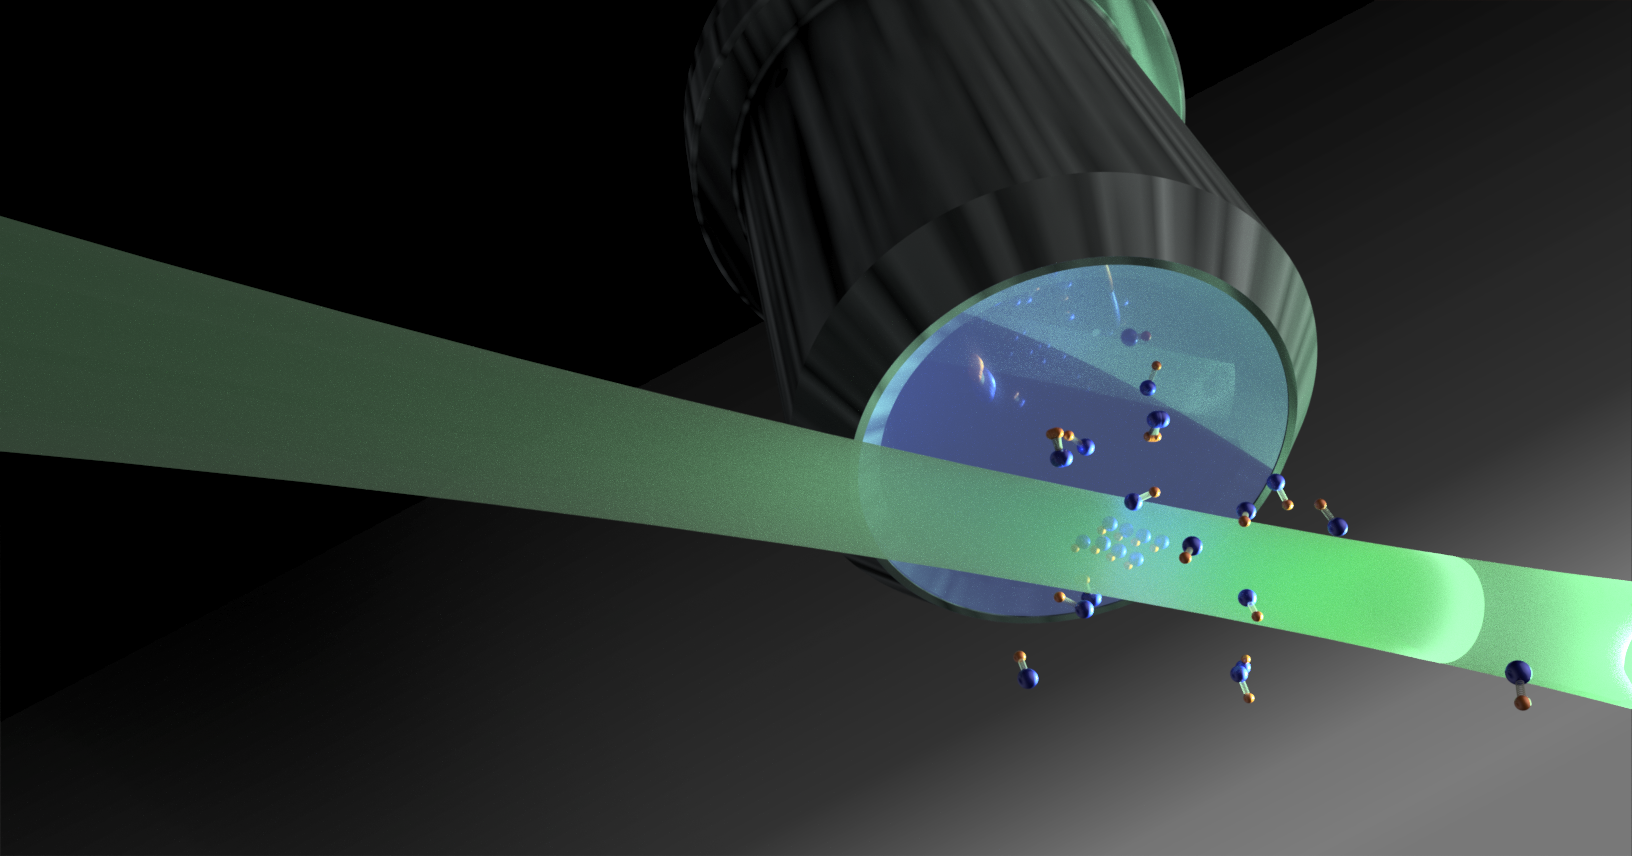
\includegraphics[width=\paperwidth]{front_bg.png}}
  }
  \setbeamercolor{title}{fg=white}
  \setbeamercolor{author}{fg=white}
  \setbeamercolor{institute}{fg=white}
  \setbeamercolor{date}{fg=white}
  \begin{frame}{}
    \titlepage
  \end{frame}
}

%% Motivation
% Quantum control of molecules has been a long-standing goal in the field of AMO,
% It is important for applications like (...).
% In our experiment, we aim to achieve this by trapping the molecule in optical tweezers
% in order to take advantage of the flexibility offered by optical tweezers.

\begin{frame}{}
  \begin{center}
    \begin{tikzpicture}
      \node at (4, 3.8) {\usebeamercolor[fg]{frametitle}{\textbf{Molecules}}};
      \node[right, align=center] at (0.7, 1.9) {
        \usebeamercolor[fg]{frametitle}{\small Precision Measurement}\\
        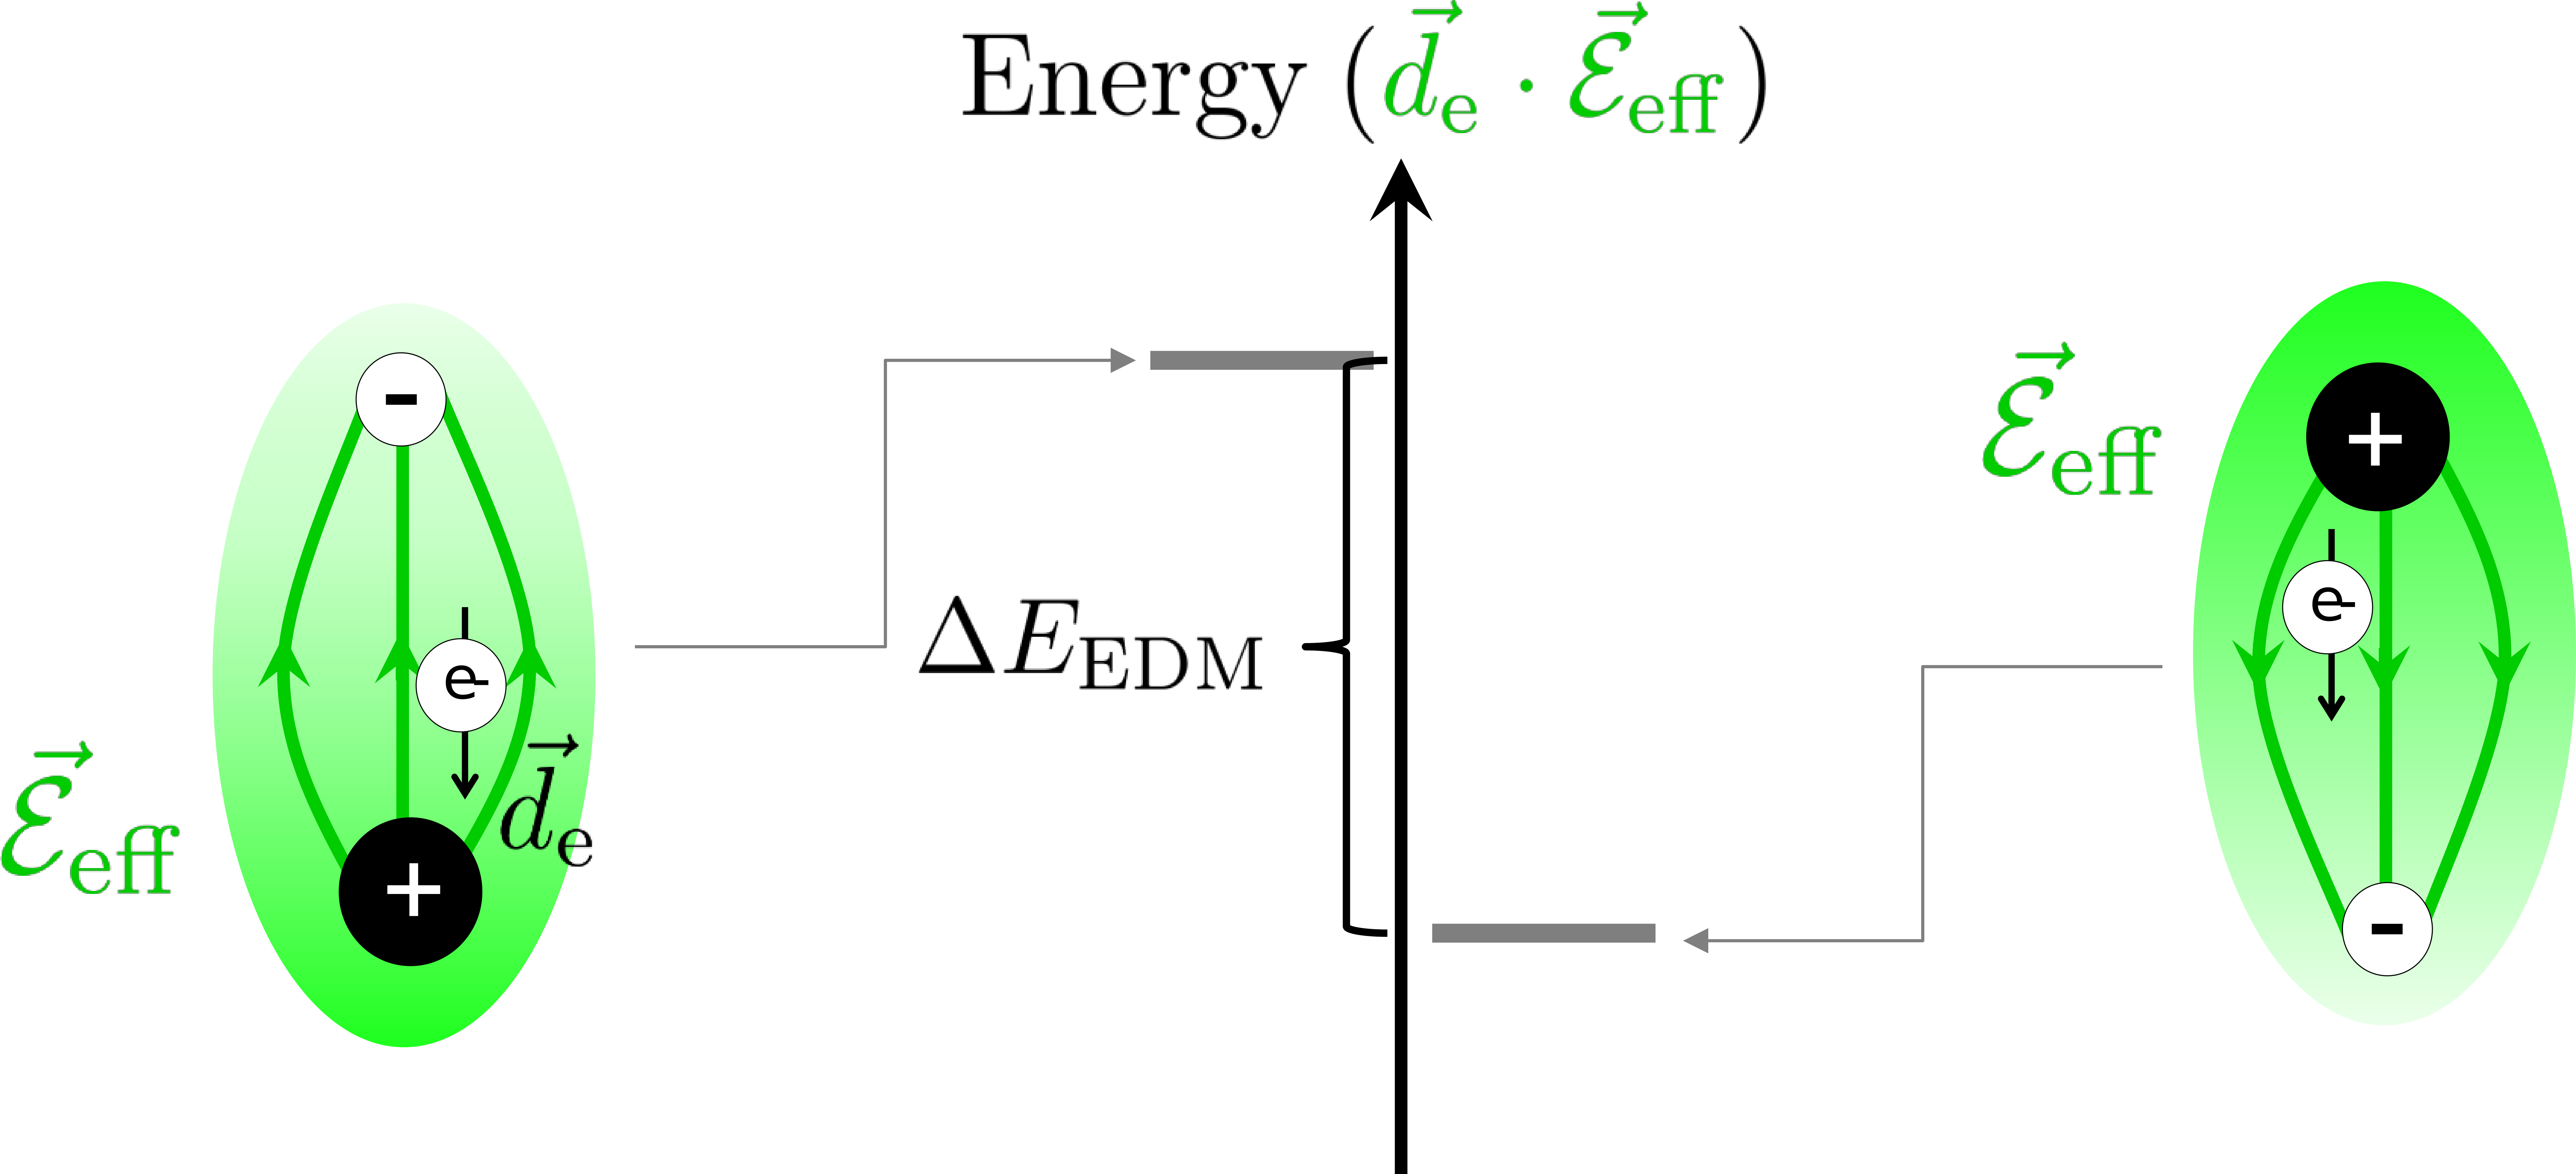
\includegraphics[width=3.6cm]{edm}\\
        {\tiny Science 343, p. 269-272 (2014)}};
      \node[right, align=center] at (1.0, -1.7) {
        \usebeamercolor[fg]{frametitle}{\small Quantum Simulation}\\
        \includegraphics[width=2.9cm]{quantum_simulation}\\
        {\tiny Nat. Phys. 2, 341 (2006)}};
      \node[right, align=center] at (4.5, 1.3) {
        \usebeamercolor[fg]{frametitle}{\small Quantum Chemistry}\\
        \includegraphics[width=2.3cm]{quantum_chemistry}\\
        {\tiny Nature 464, 1324 (2010)}};
      \node[right, align=center] at (4.2, -2.4) {
        \usebeamercolor[fg]{frametitle}{\small Quantum Computing}\\
        \includegraphics[width=2.9cm]{quantum_computing}\\
        {\tiny PRL. 97, 33003 (2006)}};
      \visible<2->{
        \node at (10, 3.8) {\usebeamercolor[fg]{frametitle}{\textbf{Optical tweezers}}};
        \begin{scope}[shift={(8.5, 1.7)}, scale=0.8]
          \only<2->{
            \mytweezer.up(0, 0)
            \mytweezer.down(2, 0.8/2.5)
            \mytweezer.up(3.8, -0.2/2.5)
            \begin{pgfonlayer}{tweezer}
              \draw[line width=1,dashed,color=cyan] (0, 0/2.5) -- (2, 0.8/2.5);
              \draw[line width=1,dashed,color=cyan] (0, 0/2.5) -- (1, -1.7/2.5);
              \draw[line width=1,dashed,color=cyan] (2, 0.8/2.5) -- (1, -1.7/2.5);
              \draw[line width=1,dashed,color=cyan] (2.9, -1.9/2.5) -- (1, -1.7/2.5);
              \draw[line width=1,dashed,color=cyan] (2.9, -1.9/2.5) -- (2, 0.8/2.5);
              \draw[line width=1,dashed,color=cyan] (3.8, -0.2/2.5) -- (2, 0.8/2.5);
              \draw[line width=1,dashed,color=cyan] (2.9, -1.9/2.5) -- (3.8, -0.2/2.5);
            \end{pgfonlayer}
            \mytweezer.down(1, -1.7/2.5)
            \mytweezer.up(2.9, -1.9/2.5)
          }
          % Mark the edge for the \only<2-> plot above so that the picture doesn't move
          \draw[white, opacity=0] (4.5, -2) -- (4.5, 2);
        \end{scope}
        \node[below, text width=4.5cm] at (10, -0.5) {\begin{itemize}
          \item Single site imaging
          \item Single site addressing
          \item Flexible geometry
          \item $\cdots$
          \end{itemize}};
      }
    \end{tikzpicture}
  \end{center}
\end{frame}

%% Ultracold molecule in tweezers
% At the highest level, there are two major approaches
% that people use to make ultracold molecules.
% 1. Direct cooling
% % which include the CaF experiment from Harvard that has recently been able to load
% % single CaF molecule in optical tweezer. (10.1126/science.aax1265)
% 2. (which we use) is to assemble the molecule from ultracold atoms cooled using
% % conventional methods.

% Understandably, the challenge for the direct cooling is to achieve
% temperature and in general quantum control comparable to what people can get
% with atoms and the challenge for the assembly approach is to form the molecule
% while maintaining the control we already have on the atom and map it onto the molecule.
% And in this talk I'll show you how we form the molecule coherently from atoms.

\begin{frame}{Ultracold molecule in tweezers}
  \begin{center}
    \begin{tikzpicture}
      \node at (-3, 4) {\usebeamercolor[fg]{frametitle}{\textbf{Direct cooling}}};
      \node[below, align=center] at (-3, 3.5) {
        \includegraphics[width=6cm]{CaF_tweezer.png}\\
        \vspace{0.5cm}
        \scriptsize Science 365, p. 1156-1158 (2019)
      };

      \visible<2->{
        \node at (3, 4) {\usebeamercolor[fg]{frametitle}{\textbf{Assembly}}};
        \begin{scope}[shift={(1.6, 3.2)}, scale=0.5]
          \shade[ball color=blue!90] (-0.8, 0.2) circle (0.45);
          \shade[ball color=orange!90] (0.3, -0.2) circle (0.3);
        \end{scope}
        \node[align=center] (atom) at (3, 3.2) {\hspace{1cm}\textbf{Ultracold atoms}};
        \begin{scope}[shift={(1.35, 1.5)}, scale=0.5]
          \shade[ball color=blue!90] (-0.2, -0.1) circle (0.45);
          \shade[ball color=orange!90] (0.2, 0.1) circle (0.3);
        \end{scope}
        \node[align=center] (molecule) at (3, 1.5) {\hspace{1cm}\textbf{Ultracold molecule}};
        \draw[blue, ->, line width=2] (atom) --
        node[right] {\small \textbf{Coherent transfer}} (molecule);
      }

      \visible<3->{
        \node at (0, 0) {\usebeamercolor[fg]{frametitle}{\underline{\textbf{Challenges}}}};
      }

      \visible<3->{
        \node[below, text width=5.5cm, align=left] at (-3, -0.8) {\begin{itemize}
          \item Temperature in tweezer
          \item Quantum control
          \end{itemize}};
      }

      \visible<4->{
        \node[below, text width=4cm, align=left] at (3, -0.7) {\begin{itemize}
          \item Creating molecules
          \item Maintain coherence
          \end{itemize}};
      }
    \end{tikzpicture}
  \end{center}
\end{frame}

%% Molecule assembly
% Using the assembly approach, we start our experiment by establishing the
% quantum control on the atom.
% This includes trapping, cooling, preparation of the internal states
% and merging the atom into a single trap which is the starting point for creating the molecule.

% At this stage, the two atoms are about as closed to each other as they can be
% from the confinement, which is ~1000 Bohr radius. However, in order to make a molecule,
% the two atoms have to be a few Bohr radius apart and this length scale difference poses the
% biggest challange for creating molecules from atoms.

\begin{frame}{}
  \begin{center}
    \begin{tikzpicture}
      \node[below,align=center] at (1.75, 4)
      {\hspace{0.5cm}\usebeamerfont{frametitle}\usebeamercolor[fg]{frametitle}{Loading}\\
        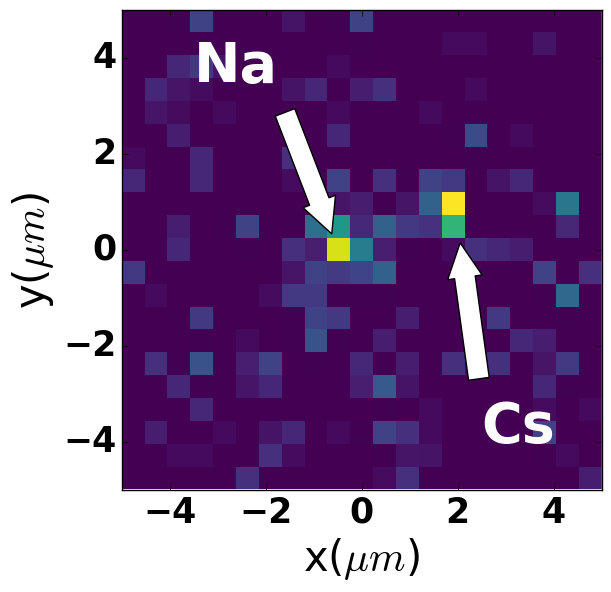
\includegraphics[width=3cm]{../../experiments/nacs_atoms/imgs/single_viridis.png}};
      \node[above,align=center] at (2, 0.36)
      {\usebeamercolor[fg]{frametitle}{\tiny{NJP. 19, 023007 (2017)}}};
      \node[below,align=center] at (2.1, 0.28)
      {\usebeamerfont{frametitle}\usebeamercolor[fg]{frametitle}{Cooling}\\
        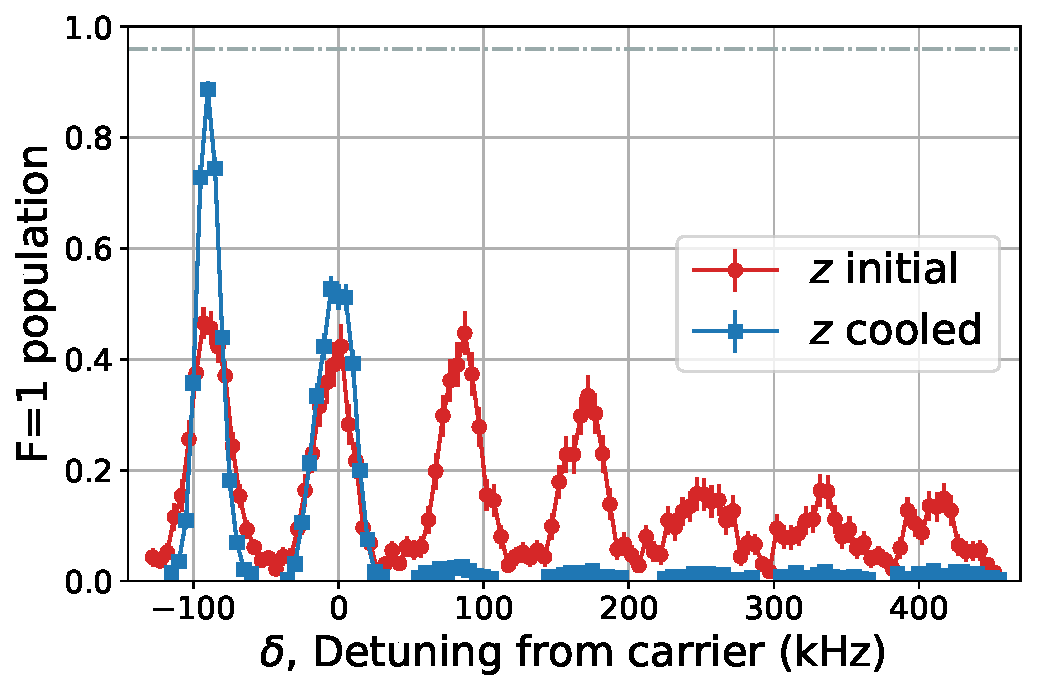
\includegraphics[width=4.2cm]{spectrum_nolabel_az.pdf}};
      \node[below,align=center] at (5.25, 3.5)
      {\usebeamerfont{frametitle}\usebeamercolor[fg]{frametitle}{Merging}};
      \node[above,align=center] at (2.2, -3.3)
      {\usebeamercolor[fg]{frametitle}{\tiny{PRA. 97, 063423 (2018)}}};
      \node[above,align=center] at (5.4, -3.1)
      {\usebeamercolor[fg]{frametitle}{\tiny{PRX. 9, 021039 (2019)}}};
      \begin{scope}[shift={(4.8, 4)}, xscale=-0.8, yscale=0.8]
        \mytweezer.drawCsTweezer(0, -3.1)
        \mytweezer.drawNaTweezer(-1, -3.1)
        \mytweezer.drawCsAtom(0.0, -3.1, 0.12)
        \mytweezer.drawNaAtom(-1.0, -3.1, 0.16)

        \mytweezer.drawCsTweezer(-1, -7.0)
        \mytweezer.drawNaAtom(-1.05, -6.87, 0.16)
        \mytweezer.drawCsAtom(-0.95, -7.13, 0.12)

        \begin{scope}[opacity=0.7]
          \draw[->,orange,line width=1.2] (-1, -3.3) -- (-1, -6.7);
          \draw[->,blue,domain=-3.3:-6.7,smooth,variable=\y,line width=1.2]
          plot ({atan((\y+4.7) * 5) / 170 - 0.5},{\y});
        \end{scope}
      \end{scope}
      \visible<2->{
        \begin{scope}[shift={(9.5, 2.5)}, scale=0.8]
          \draw[line width=1] plot[samples=200,domain=-2:2,variable=\x] ({\x + 0}, {(\x)^2 * 0.8 - 1.5});
          \draw[line width=2,orange!90!black]
          plot[samples=200,domain=-2:2,variable=\x] ({\x + 0}, {exp(-(\x)^2 * 1.3) - 0.988});
          \draw[line width=0.8] (0 - 0.8, -0.988) -- (0 + 0.8, -0.988);
          \draw[<->,line width=1] (0 - 1, 0.3) -- (0 + 1, 0.3);
          \path (0, 0.3) node[above] {$1000a_0$};
          \path (0, -1.8) node[below] {\textbf{Atom}};
        \end{scope}
        \begin{scope}[shift={(9.5, -1.5)}, scale=0.8]
          \shade[ball color=blue!90] (0, 0) circle (0.45);
          \shade[ball color=orange!90] (0.4, 0.2) circle (0.3);
          \draw[<->,line width=1] (-0.45, 0.4) -- (0.35, 0.8);
          \path (-0.05, 0.6) node[rotate=26.565,above=2pt] {$4a_0$};
          \path (0, -1) node[below] {\textbf{Molecule}};
        \end{scope}
      }
    \end{tikzpicture}
  \end{center}
\end{frame}

%% Size mismatch
% The size mismatch really necessitate a two step transfer process,
% where we would first transfer from the atomic state to an intermediate molecular state
% before using a second step to transfer to the final state and each of the steps
% now have a much reduced mismatch.
% And today I'll mostly focus on the first step starting from the atomic state
% (as you might have guessed from the title of my talk).

% The "tranditional" choice of the intermediate state is a FB molecule.
% Indeed, it also works for our system and we've recently created a single FB
% molecule in the optical tweezer that is suitable for doing the next step transfer from.
% However, this approach obviously rely on finding a good FB resonance so it is
% not very general and it may also require large B field which may not be convinient/compatible.

% What I am going to talk about today, OTOH, is a different approach that uses only
% optical transitions to go from the atomic state to a weakly-bound molecular state.
% By not relying on FB resonance, this approach is faster, does not require
% a big coil, and most importantly, we hope this can be more generally apply to
% molecules that may not have an accessible/usable FB resonance.

% It's worth pointing out that optical transfer has been previously done
% including this atomic to molecular Raman resonance.
% However, it was either done incoherently, or it relies on narrow line transition
% in Alkali earth atoms limiting the generality of the approach.

\begin{frame}{}
  \begin{center}
    \begin{tikzpicture}
      \begin{scope}[shift={(-1, 0)}, scale=0.9]
        \begin{scope}[shift={(-5, 3)}, scale=0.6]
          \draw[line width=1] plot[samples=200,domain=-2:2,variable=\x] ({\x + 0}, {(\x)^2 * 0.8 - 1.5});
          \draw[line width=2,orange!90!black]
          plot[samples=200,domain=-2:2,variable=\x] ({\x + 0}, {exp(-(\x)^2 * 1.3) - 0.988});
          \draw[line width=0.8] (0 - 0.8, -0.988) -- (0 + 0.8, -0.988);
          \draw[<->,line width=1] (0 - 1, 0.3) -- (0 + 1, 0.3);
          \path (0, 0.3) node[above] {$1000a_0$};
          \path (0, -1.8) node[below] {\small \textbf{Atom}};
        \end{scope}
        \begin{scope}[shift={(-2.2, 3)}, scale=0.6]
          \shade[ball color=blue!90] (-0.4, -0.1) circle (0.55);
          \shade[ball color=orange!90] (0.4, 0.3) circle (0.4);
          \draw[<->,line width=1] (-1.05, 0.4) -- (0.55, 1.2);
          \path (-0.25, 0.8) node[rotate=26.565,above=2pt] {$\approx 20\!-\!200a_0$};
          \path (0, -1.2) node[below,align=center] {\small \textbf{Weakly-Bound}\\\small \textbf{Molecule}};
        \end{scope}
        \begin{scope}[shift={(0, 3)}, scale=0.6]
          \shade[ball color=blue!90] (0, 0) circle (0.45);
          \shade[ball color=orange!90] (0.4, 0.2) circle (0.3);
          \draw[<->,line width=1] (-0.45, 0.4) -- (0.35, 0.8);
          \path (-0.05, 0.6) node[rotate=26.565,above=2pt] {$4a_0$};
          \path (0, -1) node[below] {\small \textbf{Molecule}};
        \end{scope}
        \visible<2->{
          \draw[line width=1, red] (-6.4, 4.35) rectangle (-0.9, 1.35);
        }
      \end{scope}
      \visible<3-4>{
        \node at (-3, 0.8) {\usebeamercolor[fg]{frametitle}{\textbf{Feshbach molecule}}};
        \node[below, align=center] at (-3.2, 0.4)
        {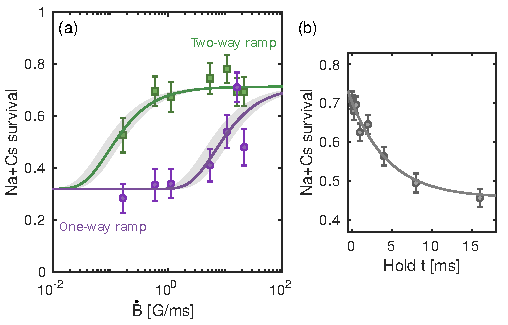
\includegraphics[width=6cm]{fb_molecules.pdf}\\
          \small{arXiv:2003.07850 (accepted by PRL)}};
        \visible<4->{
          \node[below, text width=6cm, align=left] at (3, -0.3) {\begin{itemize}
            \item Requires Feshbach resonance
            \item Usually large magnetic field
            \end{itemize}
          };
        }
      }
      \visible<5->{
        \node[below, text width=6cm, align=center] at (-3.3, 1)
        {{\usebeamercolor[fg]{frametitle}{\textbf{Optical transfer}}}\\
          \begin{itemize}
          \item More general
          \item Faster
          \end{itemize}
        };
      }
      \visible<6->{
        \node[below, text width=6cm, align=left] at (3.1, 4)
        {
          {\usebeamercolor[fg]{frametitle}{Previous results}}\\
          {\footnotesize $\mathrm{Rb_2}$}
          {\tiny \usebeamercolor[fg]{frametitle}{Science 287, p. 1016-1019 (2000)}}\\
          \phantom{{\footnotesize $\mathrm{Rb_2}$}}
          {\tiny \usebeamercolor[fg]{frametitle}{PRL. 93, 073002 (2004)}}\\
          \includegraphics[width=3.5cm]{Rb2_raman.png}\\
          {\footnotesize $\mathrm{Sr_2}$}
          {\usebeamercolor[fg]{frametitle}{\tiny PRL. 96, 203201 (2006)}}\\
          {\footnotesize $\mathrm{NaCs}$}
          {\usebeamercolor[fg]{frametitle}{\tiny PRX. 9, 021039 (2019)}}\\
          \includegraphics[width=3.5cm]{old_raman_transfer.pdf}
        };
      }
      \visible<7->{
        \node[below, text width=6cm, align=center] at (-3.3, -1.3)
        {
          {\usebeamercolor[fg]{frametitle}{Limitations so far}}\\
          \begin{itemize}
          \item Incoherent due to scattering
          \item Rely on narrow line optical transition
          \end{itemize}
        };
      }
    \end{tikzpicture}
  \end{center}
\end{frame}

%% Raman scheme
% The scheme we use is actually very simple.
% After cooling the atoms into th motional ground state, we shine a pair of
% lasers detuned from an excited state to drive a Raman transition into the
% molecular state and we usually target the least bound molecular state
% which is the most similar to the initial state.

% Since one of the major challenges is the mismatch of the wavefunction size,
% it makes sense to pick a molecular state that is as "big" as possible,
% i.e. the molecular states that are closed to the threshold or even the first bound state.
% Indeed, this is what all previous attempts use and this enable them to drive the Raman
% transition with relative ease.
% However, these states are very closely spaced, and in case of the excited state, this makes
% it hard to detune and reduce the scattering, which ultimately limits the coherence,
% as I metioned previously.
% If we instead use an excited state that is more deeply bound. Even though
% the Raman coupling is smaller due to a worse size mismatch, since the states are
% more sparsely spaced, we can now detune further to reduce the scattering
% without worrying about hitting another state.

% It may not be obvious if the deeply bound state offers enough coupling,
% or if it reduces the scattering more than the reduction of the Raman coupling.
% That's why we did a calculation:
% % Here you see the Raman Rabi frequency and the scattering rate calculated for
% % Raman beam detuned from two different states.
% % .....
% % Showing that even though at the same deuning the Raman Rabi frequecy is lower for the
% % deeply bound state, we can detune more and win on the Raman Rabi frequency/scattering rate
% % ratio.

\begin{frame}[t]{Raman transfer}
  \begin{center}
    \vspace{-0.9cm}
    \begin{tikzpicture}
      \begin{scope}[scale=0.8]
        \draw[->,line width=1.2] (0, 0) -- (0, 8);
        \node[above,rotate=90] at (0, 4) {Energy};
        \draw[->,line width=1.2] (0, 0) -- (5.4, 0);
        \node[below] at (2.7, -0.1) {Internuclear distance};

        \draw[cyan!85!blue] ({(1.0269 + 0.25) * 0.7}, 2.5) -- (7.25 * 0.7, 2.5);

        \draw[line width=1.1,cyan!85!blue]
        plot[samples=200,domain=0.96:7,variable=\x]
        ({(\x + 0.25) * 0.7}, {(6.8*\x^(-3.4)-6.5*\x^(-1.7)) * 1.3 + 2.5});

        \draw[line width=1.1,red]
        plot[samples=200,domain=1:7.5,variable=\x]
        ({(\x - 0.75) * 0.7}, {(9.2*\x^(-2.5)-9.0*\x^(-1.3)) * 1.3 + 7.5});
        \node[above right,red] at (0.55 * 0.7, 7.2) {$c^3\Sigma^+$};

        \visible<-2,4>{
          \draw[red] ({(1.1102 - 0.75) * 0.7}, -0.69 * 1.3 + 7.5) --
          ({(6.5 - 0.75) * 0.7}, -0.69 * 1.3 + 7.5);
        }
        \visible<3->{
          \draw[red] ({(1.4 - 0.75) * 0.7}, -1.8 * 1.3 + 7.5) --
          ({(2.5 - 0.75) * 0.7}, -1.8 * 1.3 + 7.5);
        }
        \visible<-2>{
          \draw[black!40,dashed,line width=1] ({(0.9 - 0.75) * 0.7}, -0.77 * 1.3 + 7.5) --
          ({(7 - 0.75) * 0.7}, -0.77 * 1.3 + 7.5);
        }
        \visible<3>{
          \draw[black!40,dashed,line width=1] ({(1.2 - 0.75) * 0.7}, -2 * 1.3 + 7.5) --
          ({(3 - 0.75) * 0.7}, -2 * 1.3 + 7.5);
        }
        \visible<4->{
          \draw[blue, line width=1]
          ({(1.1102 - 0.75) * 0.7 - 0.15}, -0.69 * 1.3 + 7.5 - 0.15) rectangle
          ({(6.5 - 0.75) * 0.7 + 0.15}, -0.69 * 1.3 + 7.5 + 0.15);
          \coordinate (ThresholdHighlight)
          at ({(6.5 - 0.75) * 0.7 + 0.25}, -0.69 * 1.3 + 7.5 - 0.08);
          \draw[blue, line width=1]
          ({(1.4 - 0.75) * 0.7 - 0.15}, -1.8 * 1.3 + 7.5 - 0.15) rectangle
          ({(2.5 - 0.75) * 0.7 + 0.15}, -1.8 * 1.3 + 7.5 + 0.15);
          \coordinate (DeepHighlight)
          at ({(2.5 - 0.75) * 0.7 + 0.25}, -1.8 * 1.3 + 7.5);
        }

        \mytweezer.drawNaAtom(6.55 * 0.7, 2.6, 0.12)
        \mytweezer.drawCsAtom(7.05 * 0.7, 2.6, 0.10)

        \draw[cyan!85!blue] ({(1.0793 + 0.25) * 0.7}, -0.28 * 1.3 + 2.5) -- ({(6 + 0.25) * 0.7}, -0.28 * 1.3 + 2.5);
        \mytweezer.drawNaAtom(4.08 * 0.7, -0.19  * 1.3 + 2.5, 0.12)
        \mytweezer.drawCsAtom(4.25 * 0.7, -0.19  * 1.3 + 2.5, 0.10)

        \visible<-2>{
          \draw[->,blue!50!orange,line width=0.8] (6.8 * 0.7, 2.7)
          -- node[right] {$\Omega_{up}$} ({(3.5 - 0.75) * 0.7}, -0.8 * 1.3 + 7.5);
          \draw[->,green!80!black,line width=0.8] ({(3.45 - 0.75) * 0.7}, -0.8 * 1.3 + 7.5)
          -- node[left] {$\Omega_{down}$} (4.165 * 0.7, -0.12 * 1.3 + 2.5);
        }
        \visible<3>{
          \draw[->,blue!50!orange,line width=0.8] (6.8 * 0.7, 2.7)
          -- node[right] {$\Omega_{up}$} ({(2.8 - 0.75) * 0.7}, -2 * 1.3 + 7.5);
          \draw[->,green!80!black,line width=0.8] ({(2.75 - 0.75) * 0.7}, -2 * 1.3 + 7.5)
          -- node[left] {$\Omega_{down}$} (4.165 * 0.7, -0.12 * 1.3 + 2.5);
        }
      \end{scope}
      \visible<2-3>{
        \node[below, text width=5.4cm, align=center] at (8.13, 6.8)
        {
          {\usebeamercolor[fg]{frametitle}{\textbf{Near threshold states}}}\\
          \vspace{0.2cm}
          \begin{itemize}
          \item Stronger coupling\\
            ($\Omega_{up}$ and $\Omega_{down}$)
          \item Closely spaced
          \item Fast scattering
          \end{itemize}
        };
      }
      \visible<3>{
        \node[below, text width=5.4cm, align=center] at (8.13, 2.7)
        {
          {\usebeamercolor[fg]{frametitle}{\textbf{Deeply bound states}}}\\
          \vspace{0.2cm}
          \begin{itemize}
          \item Weaker coupling
          \item Sparsely spaced
          \item Allow larger detuning
          \item Slower scattering
          \end{itemize}
          {\tiny \usebeamercolor[fg]{frametitle}{arXiv:1701.03121(2017)}}
        };
      }
      \visible<4>{
        \node[below, text width=5.4cm, align=center] (ThresholdPlot) at (8.13, 7.5)
        {
          {\usebeamercolor[fg]{frametitle}{\textbf{Near threshold states}}}
          \includegraphics[width=5.4cm]{imgs/raman_vh.pdf}
        };
        \node[below, text width=5.4cm, align=center] (DeepPlot) at (8.13, 3.2)
        {
          {\usebeamercolor[fg]{frametitle}{\textbf{Deeply bound states}}}
          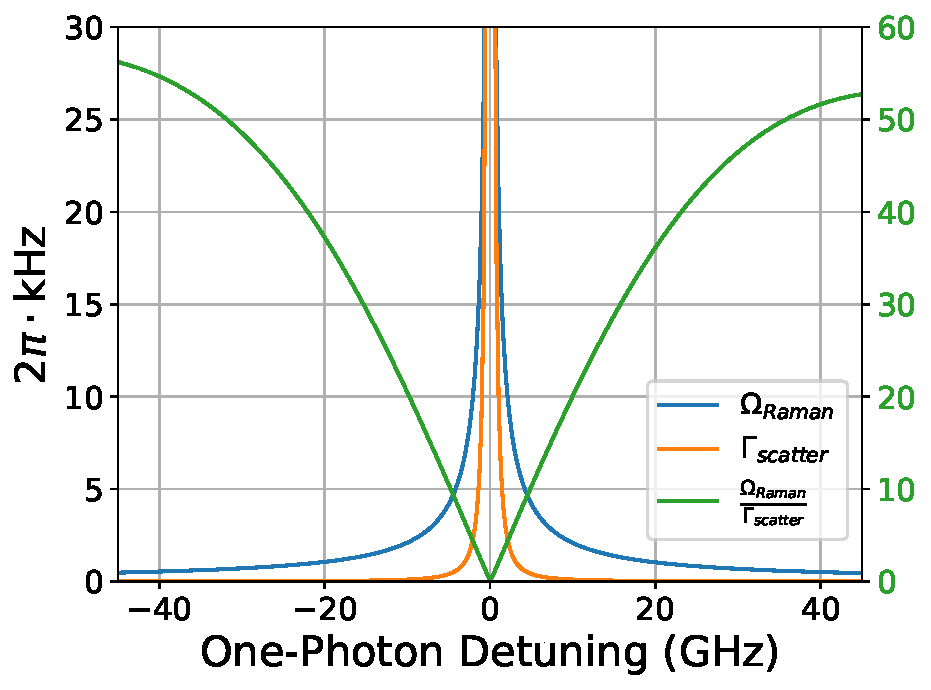
\includegraphics[width=5.4cm]{imgs/raman_v0.pdf}
        };
        \draw[->, blue, line width=2] (ThresholdPlot) -- (ThresholdHighlight);
        \draw[->, blue, line width=2] (DeepPlot) -- (DeepHighlight);
      }
    \end{tikzpicture}
  \end{center}
\end{frame}

%% Experiment
% Based on the comparison, we selected the ground vibrational state
% in the excited state (v=0), which we have already observed previously.
% And for the ground molecular state, the binding energy was predicted as
% ~770 MHz by Jeremy Hutson from Durham, based on our interaction shift
% and FB measurement. (Phys. Rev. Research 2, 023108 (2020))

% Thanks to the prediction, it didn't take too long for us to find the resonance.
% (Show Raman spectrum) which was ~1MHz from the prediction.
% More importantly though, this is taken with a 0.1 ms pulse time and we got a FWHM of
% 8.4 kHz which is what you'll expect from a Fourier limited linewidth.
% This suggests that we are at least very closed to the coherent regime where the
% Raman Rabi frequency exceeds the scattering rate.
% Next we switched to scanning the time on resonance.
% See oscillation!!

\begin{frame}[t]{Experiment}
  \begin{center}
    \vspace{-0.9cm}
    \begin{tikzpicture}
      \visible<-4>{
        \begin{scope}[shift={(-5.5, -3.5)}, scale=0.8]
          \draw[->,line width=1.2] (0, 0) -- (0, 8);
          \node[above,rotate=90] at (0, 4) {Energy};
          \draw[->,line width=1.2] (0, 0) -- (5.4, 0);
          \node[below] at (2.7, -0.1) {Internuclear distance};

          \draw[line width=1.1,cyan!85!blue]
          plot[samples=200,domain=0.96:7,variable=\x]
          ({(\x + 0.25) * 0.7}, {(6.8*\x^(-3.4)-6.5*\x^(-1.7)) * 1.3 + 2.5});

          \draw[line width=1.1,red]
          plot[samples=200,domain=1:7.5,variable=\x]
          ({(\x - 0.75) * 0.7}, {(9.2*\x^(-2.5)-9.0*\x^(-1.3)) * 1.3 + 7.5});
          \node[above right,red] at (0.55 * 0.7, 7.2) {$c^3\Sigma^+$};

          \draw[red] ({(1.4 - 0.75) * 0.7}, -1.8 * 1.3 + 7.5) --
          ({(2.5 - 0.75) * 0.7}, -1.8 * 1.3 + 7.5) node[right=0.2] {\scriptsize $v=0$};
          \draw[black!40,dashed,line width=1] ({(1.2 - 0.75) * 0.7}, -2 * 1.3 + 7.5) --
          ({(3 - 0.75) * 0.7}, -2 * 1.3 + 7.5);

          \draw[cyan!85!blue] ({(1.0269 + 0.25) * 0.7}, 2.5) -- (7.25 * 0.7, 2.5);
          \mytweezer.drawNaAtom(6.55 * 0.7, 2.6, 0.12)
          \mytweezer.drawCsAtom(7.05 * 0.7, 2.6, 0.10)

          \draw[cyan!85!blue] ({(1.0793 + 0.25) * 0.7}, -0.28 * 1.3 + 2.5) -- ({(6 + 0.25) * 0.7}, -0.28 * 1.3 + 2.5);
          \mytweezer.drawNaAtom(4.08 * 0.7, -0.19  * 1.3 + 2.5, 0.12)
          \mytweezer.drawCsAtom(4.25 * 0.7, -0.19  * 1.3 + 2.5, 0.10)

          \draw[->,blue!50!orange,line width=0.8] (6.8 * 0.7, 2.7)
          -- node[right] {$\Omega_{up}$} ({(2.8 - 0.75) * 0.7}, -2 * 1.3 + 7.5);
          \draw[->,green!80!black,line width=0.8] ({(2.75 - 0.75) * 0.7}, -2 * 1.3 + 7.5)
          -- node[left] {$\Omega_{down}$} (4.165 * 0.7, -0.12 * 1.3 + 2.5);

          \draw[->,cyan!55!blue, line width=1] (5.1 * 0.7, 3) -- (5.1 * 0.7, 2.5);
          \draw[<-,cyan!55!blue, line width=1] (5.1 * 0.7, -0.28 * 1.3 + 2.5)
          -- (5.1 * 0.7, -0.28 * 1.3 + 2)
          node[below, align=center] {\scriptsize $\approx771\mathrm{MHz}$\\
            \scriptsize by Jeremy Hutson.};
        \end{scope}
      }
      \visible<2> {
        \node[below] at (2.6, 4) {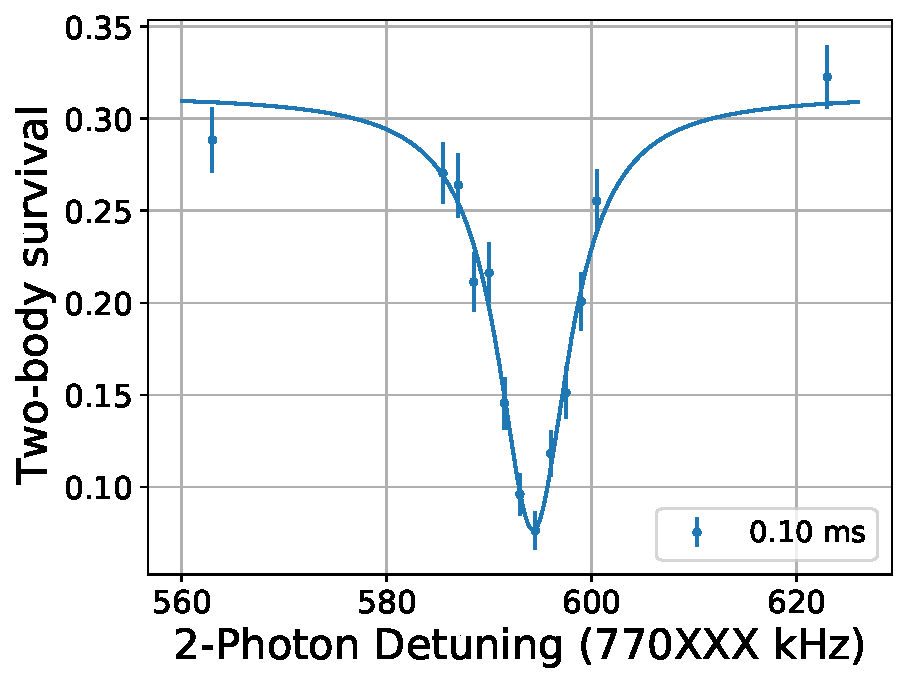
\includegraphics[width=5.5cm]{../../experiments/nacs_202003/imgs/fit_20200326_005204_raman_3322_2_damop_f.pdf}};
      }
      \visible<3-> {
        \node[below] at (2.6, 4) {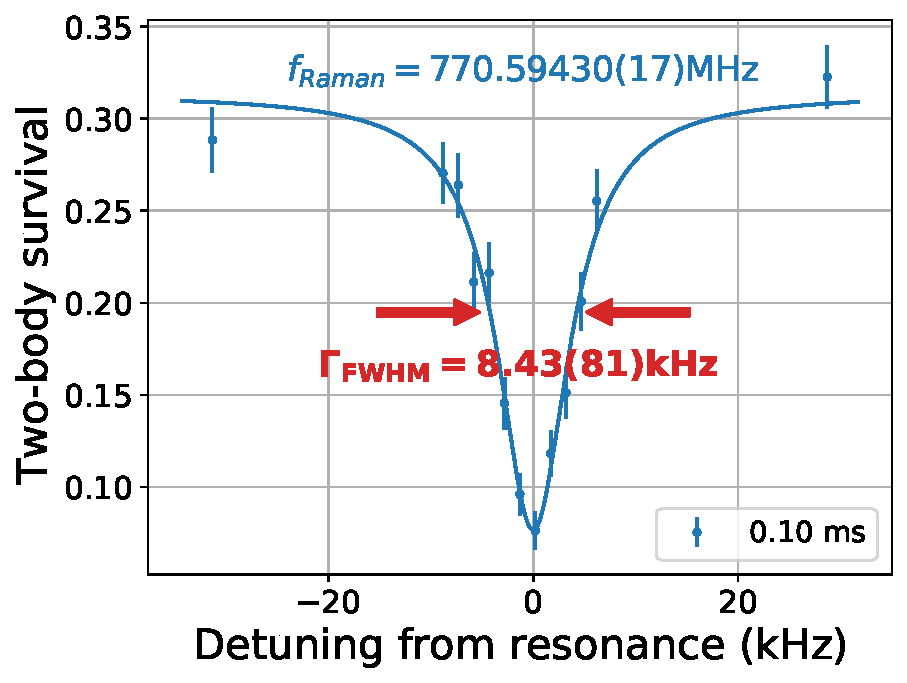
\includegraphics[width=5.5cm]{../../experiments/nacs_202003/imgs/fit_20200326_005204_raman_3322_2_damop_f_text.pdf}};
      }
      \visible<4-> {
        \node[below] at (2.6, -0.5) {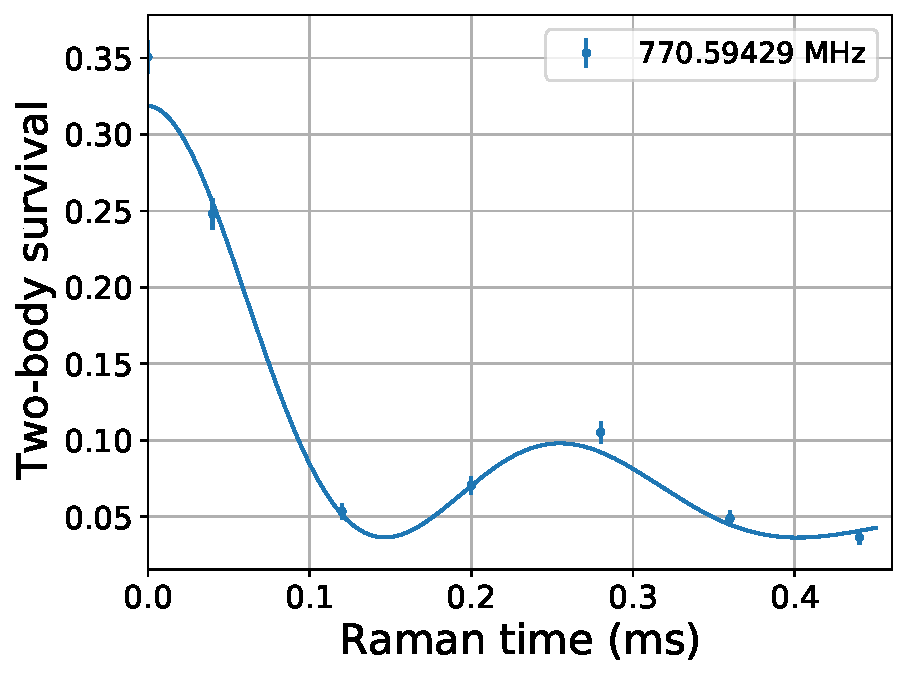
\includegraphics[width=5.5cm]{../../experiments/nacs_202003/imgs/fit_20200326_005204_raman_3322_2_damop_t.pdf}};
      }
      \visible<5-> {
        \node[below, text width=5.5cm, align=center] at (-3, 3.4)
        {
          \begin{itemize}
          \item Transferred $50\%$ of ground state atom to molecule.
          \item<6-> $>50\%$ of molecule in motional ground state.
          \end{itemize}
        };
        \node[below] at (-3.2, 0.5) {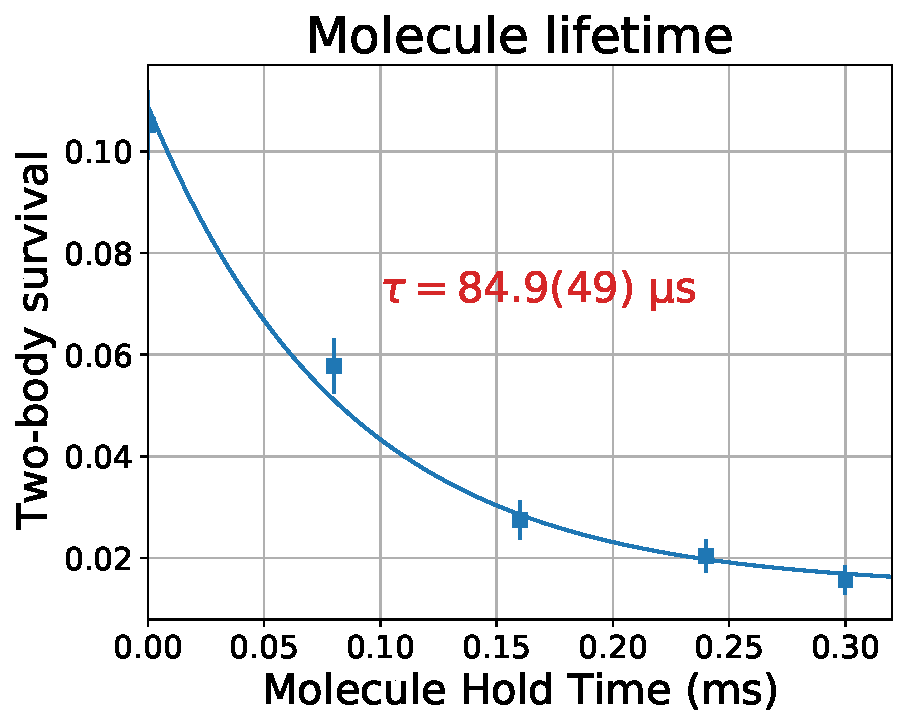
\includegraphics[width=5.3cm]{../../experiments/nacs_202003/imgs/fit_20200326_005204_raman_3322_2_damop_m_t.pdf}};
      }
    \end{tikzpicture}
  \end{center}
\end{frame}

%% Next
% We are currently working on, with obvious difficulty, improving our signal,
% by improving the fidelity of our sequence and by tweaking transfer parameters.
% It's also worth noting that the contrast isn' great, to put it mildly, much
% worse than the prediction from the Raman Rabi frequency/scattering ratio from calculation.
% Fortunately, as I mentioned earlier, our parallel effort for making FB molecule
% also succeeded recently and is showing a decent lifetime of 4-5 ms,
% so we'll be able to work on transfering to molecular ground state from FB molecule
% as we are investigating the lifetime issue.

\begin{frame}[t]{Conclusion and Outlook}
  \begin{center}
    \begin{tikzpicture}
      \node[below, text width=5.7cm, align=center] at (-3, 4) {
        \begin{block}{}
          \begin{itemize}
          \item<1-> Demonstrated formation of weakly-bound NaCs
            molecules while maintaining quantum control.
          \item<2-> Improve signal contrast.
          \item<3-> Feshbach molecule\\
            {\small $\left(\tau=4.7(7)\ \mathrm{ms}\right)$}\\
            \vspace{0.2cm}
            \small{arXiv:2003.07850}
          \end{itemize}
        \end{block}
      };
      \visible<2-> {
        \node[below] at (3, 3.4) {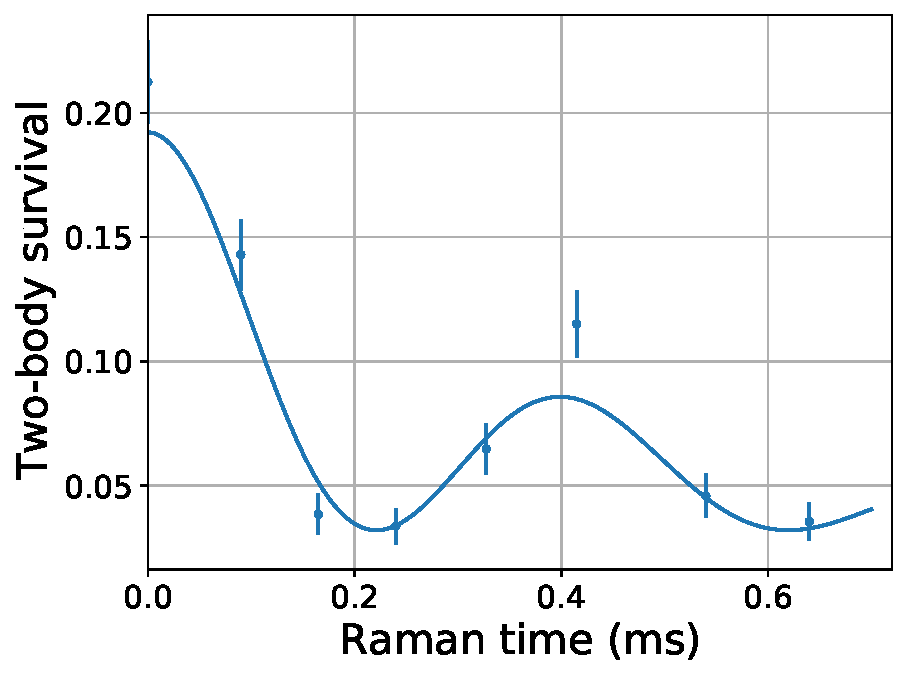
\includegraphics[width=5.5cm]{../../experiments/nacs_202005/imgs/fit_20200524_161707_raman_3322_damop_t.pdf}};
      }
      \visible<4->{
        \node[below, align=center] at (0, -1.2) {
          \textbf{Poster Q01.00108}
        };
      }
    \end{tikzpicture}
  \end{center}
\end{frame}

\begin{frame}{}
\end{frame}

\end{document}
